\begin{SCfigure}[3]
  \centering
  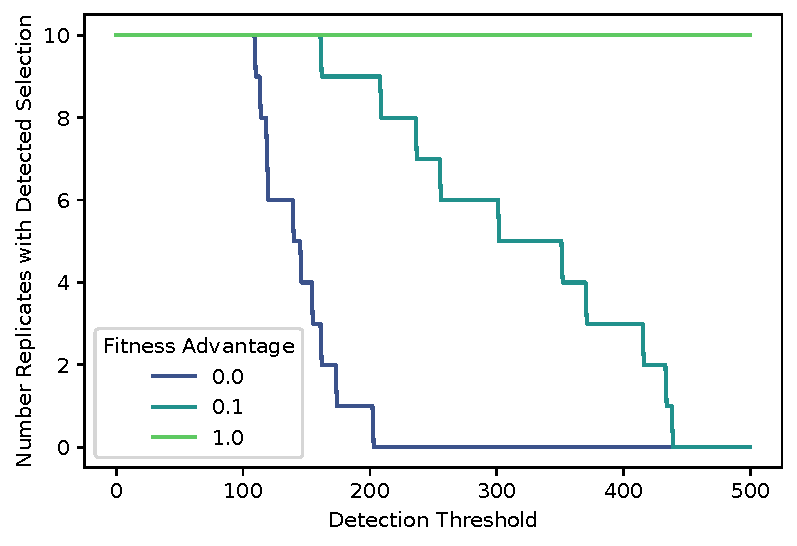
\includegraphics[width=0.6\textwidth]{notebooks/notebooks/teeplots/hue=fitness-advantage+viz=lineplot-detection+x=threshold+y=replicate-count+ext=}
  \caption{
    Gene selection detection rates by threshold for each fitness advantage level among 10 replicates.
    Fitness advantage 0.0 inferred no selective benefit, so all selection detections on this treatment are false positives.
    Detection threshold 200 distinguishes treatment 0.0 and 0.1 with one false positive and one false negative.
  }
  \label{fig:selection-sensitivity-specificity}
\end{SCfigure}
